\documentclass[11pt, oneside]{article}   	% use "amsart" instead of "article" for AMSLaTeX format
\usepackage{geometry}                		% See geometry.pdf to learn the layout options. There are lots.
\geometry{letterpaper}                   		% ... or a4paper or a5paper or ... 
%\geometry{landscape}                		% Activate for for rotated page geometry
%\usepackage[parfill]{parskip}    		% Activate to begin paragraphs with an empty line rather than an indent
\usepackage{graphicx}				% Use pdf, png, jpg, or eps§ with pdflatex; use eps in DVI mode
								% TeX will automatically convert eps --> pdf in pdflatex		
\usepackage{amssymb}
\usepackage{amsmath}
\usepackage{subfigure}
\usepackage{epsfig}	


\title{PHY566 Group Assignment \\ Diffusion}
\author{Group A}
%\date{}							% Activate to display a given date or no date

\begin{document}
\maketitle
\section{Diffusion Equation}
In this section, we will solve the diffusion problem both analytically and numerically given the initial density distribution.
\subsection{Part(a)}
In this section, the the spatial expectation value for $\left \langle x(t)^2 \right\rangle$ is determined analytically, given a 1D Normal Distribution$\rho(x,t)$.

\begin{equation*}
\rho(x,t)=\frac{1}{\sqrt{2\pi \sigma(t)^2}}e^{-\frac{x^2}{2\sigma(t)^2}}
\end{equation*}

In general, the expected value of a measurable function of $x$, $g(x)$, given that x has a probability density function $f(x)$, is given by the inner product of f and g.
\begin{equation*}
\left \langle g(x) \right\rangle= \int_{-\infty}^{\infty} g(x)f(x)\, \mathrm{d}x
\end{equation*}

In this case, we substitute $g(x)$, and$f(x)$ with $x(t)^2$ and $\rho(x,t)$ receptively. For every instant, t can be regarded as a constant in the integrand, hence the expected value for $x^2$ is a function of t.

\begin{equation*}
\left \langle x^2 \right\rangle= \int_{-\infty}^{\infty} x^2\frac{1}{\sqrt{2\pi \sigma(t)^2}}e^{-\frac{x^2}{2\sigma(t)^2}}\, \mathrm{d}x=\sigma(t)^2
\end{equation*}

\subsection{Part(b)}
In this subsection a program to solve the 1D diffusion equation using the finite difference form with a diffusion constant D = 2, with an initial density profile that is sharply peaked around x = 0, but extends over a few grid sites (box profile). To avoid the determination of the number of  particles  that are involved in this diffusion system, we use the notion of probability to study such system. Figure \ref{fig1} illustrates the initial probability density.

\begin{figure}[htbp]
\begin{center}
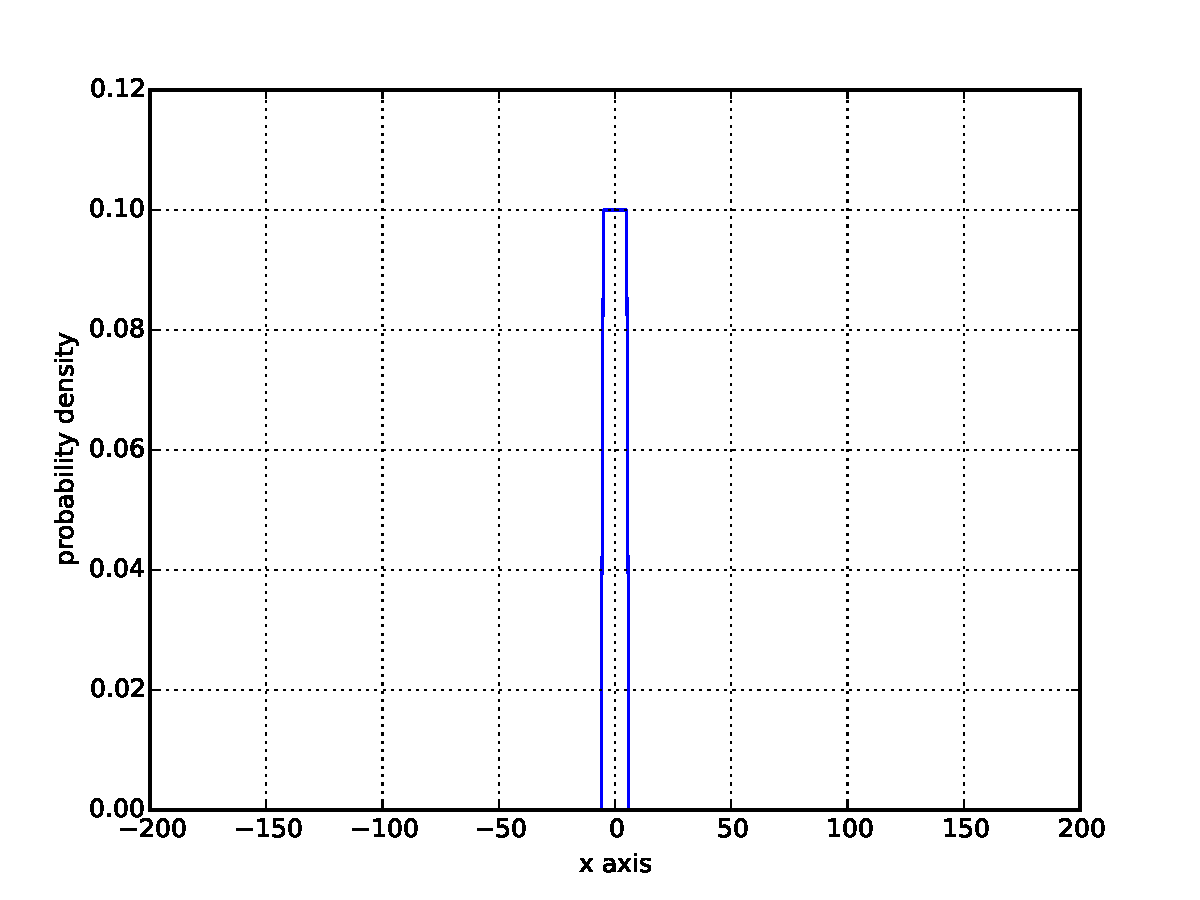
\epsfig{file=initial.pdf,scale=0.6}
\caption{{\bf  Initial probability density that is sharply peaked around x = 0, but extends over a few grid sites (box profile)}}
\label{fig1}
\end{center}
\end{figure}

Then we apply the finite difference form of the diffusion equation to solve the problem numerically.

\begin{equation*}
\rho(t+dt,x)=\rho(t,x)+D\frac{\Delta t}{{\Delta x}^2}[\rho(t,x+dx)+\rho(t,x-dx)-2\rho(t,x)]
\end{equation*}

After that, we fit the calculated densities at later time equal to 50s, 100s, 300s, 500s and 900s corresponding to a Normal Distribution with $\sigma(t)=\sqrt{2Dt}$. Figure \ref{fig2} shows the results.

\begin{figure}[htbp]
\begin{center}
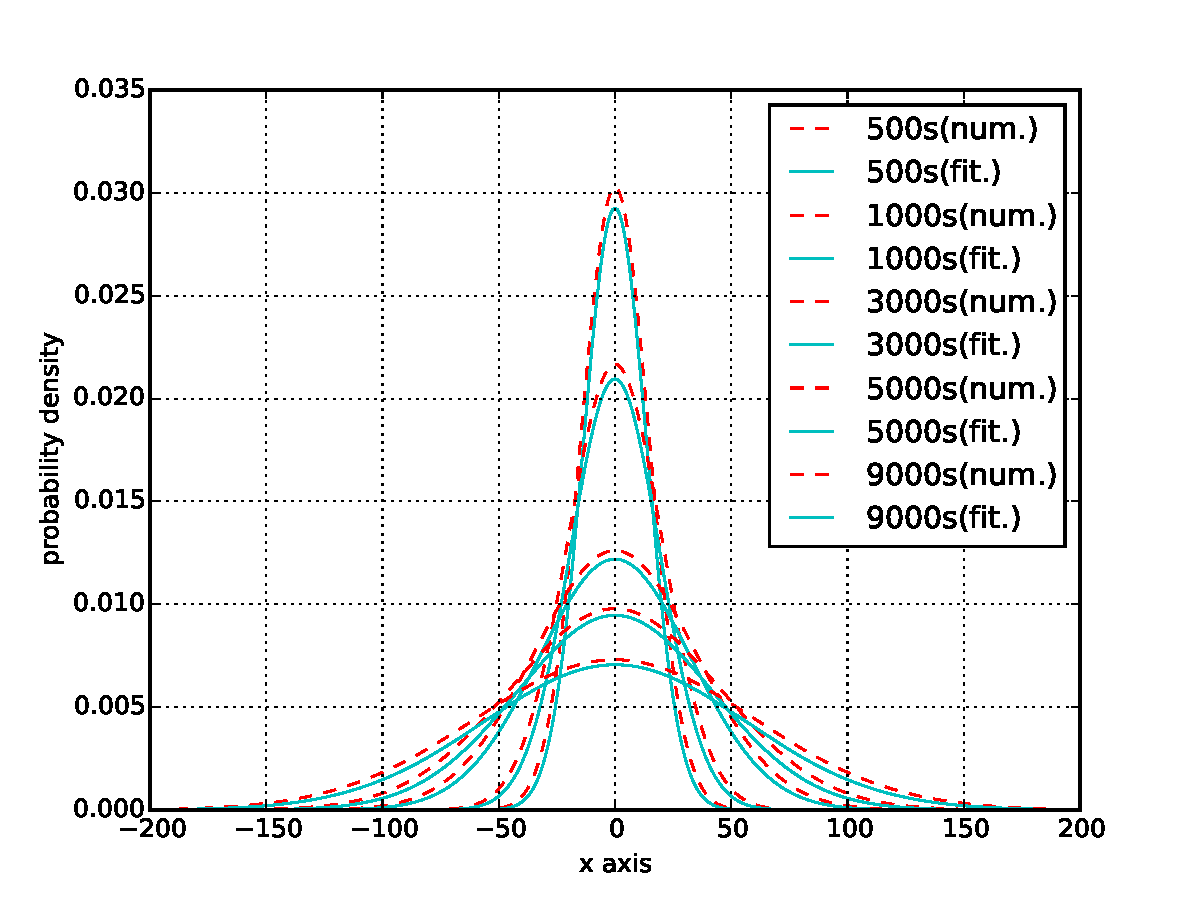
\epsfig{file=fit.pdf,scale=0.6}
\caption{{\bf   Numerically calculated probability densities with the fitting line at different times }}
\label{fig2}
\end{center}
\end{figure}

As it can be seen from raw eyes that all the numerically calculated densities can be fitted well by the the normal distribution with $\sigma(t)=\sqrt{2Dt}$.

We could also compare the fitting parameter with the idea Normal Distribution with $\sigma(t)=\sqrt{2Dt}$. Table\ref{table1} contains these values. By comparing the analytical and fit results we can verified that the numerically calculated density profile corresponds to a Normal Distribution with $\sigma(t)=\sqrt{2Dt}$ at later times. 

\begin{table}[htdp]
\caption{Analytical and fit parameters for density distribution}
\begin{center}
\begin{tabular}{l*{8}{c}r}
Time[s]              & $\mu$(analytical) & $\mu$(numerical)& $\sigma$(analytical) &$\sigma$(numerical)&  \\
\hline
500			&0	& -1.74$\times10^{-8}$ 	&14.14		&13.63  \\
1000			&0	&-1.21$\times10^{-8}$	&20.00		&19.04   \\
3000			&0 	& -2.01$\times10^{-8}$ 	&34.64		&32.71   \\
5000			&0 	& 1.19$\times10^{-8}$ 	&44.72		&42.15  \\
9000			&0 	& -2.74$\times10^{-8}$ 	&60.00		&56.49	\\
\end{tabular}
\end{center}
\label{table1}
\end{table}


\end{document}  